% The two ways of associating gamma_1 * gamma_2 * gamma_3 differ only in speed.
% Source: book/tex/topology/fundamental-group.tex (§ Fusing paths together).
\documentclass[border=2mm]{standalone}
\usepackage{tikz}
\begin{document}
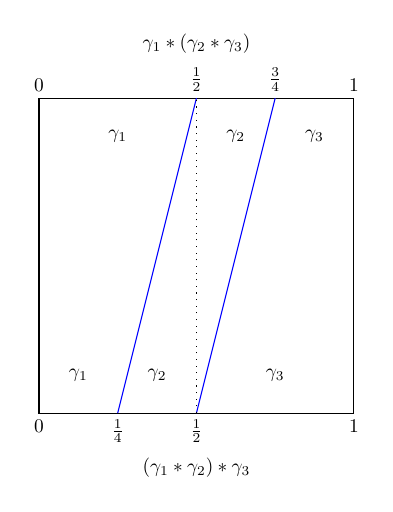
\begin{tikzpicture}[scale=4]
  \draw (0,0) rectangle (1,1);
  % bottom subdivision: 1/4, 1/2
  \foreach \x/\l in {0/0, 0.25/{\frac14}, 0.5/{\frac12}, 1/1}
    \node[below,scale=0.7] at (\x,0) {$\l$};
  % top subdivision: 1/2, 3/4
  \foreach \x/\l in {0/0, 0.5/{\frac12}, 0.75/{\frac34}, 1/1}
    \node[above,scale=0.7] at (\x,1) {$\l$};
  \node[scale=0.7] at (0.125,0.12) {$\gamma_1$};
  \node[scale=0.7] at (0.375,0.12) {$\gamma_2$};
  \node[scale=0.7] at (0.75,0.12) {$\gamma_3$};
  \node[scale=0.7] at (0.25,0.88) {$\gamma_1$};
  \node[scale=0.7] at (0.625,0.88) {$\gamma_2$};
  \node[scale=0.7] at (0.875,0.88) {$\gamma_3$};
  \node[above,scale=0.7] at (0.5,1.12) {$\gamma_1\ast(\gamma_2\ast\gamma_3)$};
  \node[below,scale=0.7] at (0.5,-0.12) {$(\gamma_1\ast\gamma_2)\ast\gamma_3$};
  \draw[blue] (0.25,0) -- (0.5,1);
  \draw[blue] (0.5,0) -- (0.75,1);
  \draw[dotted] (0.5,0) -- (0.5,1);
\end{tikzpicture}
\end{document}
